\section{Faceted Framework: Process, Modifiers, and Evidence}

The framework is faceted, not a single MECE tree. Its first facet provides narrative order. P1 contains solid-state\slash precursor-control, solution-mediated, and coprecipitation\slash combustion powder routes. P2 separates Li-sublattice substitution, Zr-site or multi-element substitution, and stoichiometry\slash defect\slash phase questions. P3 separates pressureless schedules, pressure\slash field\slash ultrafast assistance, and low-temperature or additive-assisted densification. P4 contains phase\slash microstructure and transport readouts. These are primary reading anchors, not claims that a paper changes only one variable.

The second facet attaches modifiers across that chain: dopant identity and nominal site; starting lithium inventory and firing-stage lithium supply; crucible, cover powder, atmosphere, and exposure; and sintering additives or intergranular products. The third facet records evidence needed for comparison: composition and powder-route fields, thermal-process fields, structure\slash transport measurement fields, and replication or scale fields. This separation prevents an additive, for example, from being misdrawn as a serial stage between powder and pellet.

\begin{figure*}[t]
\centering
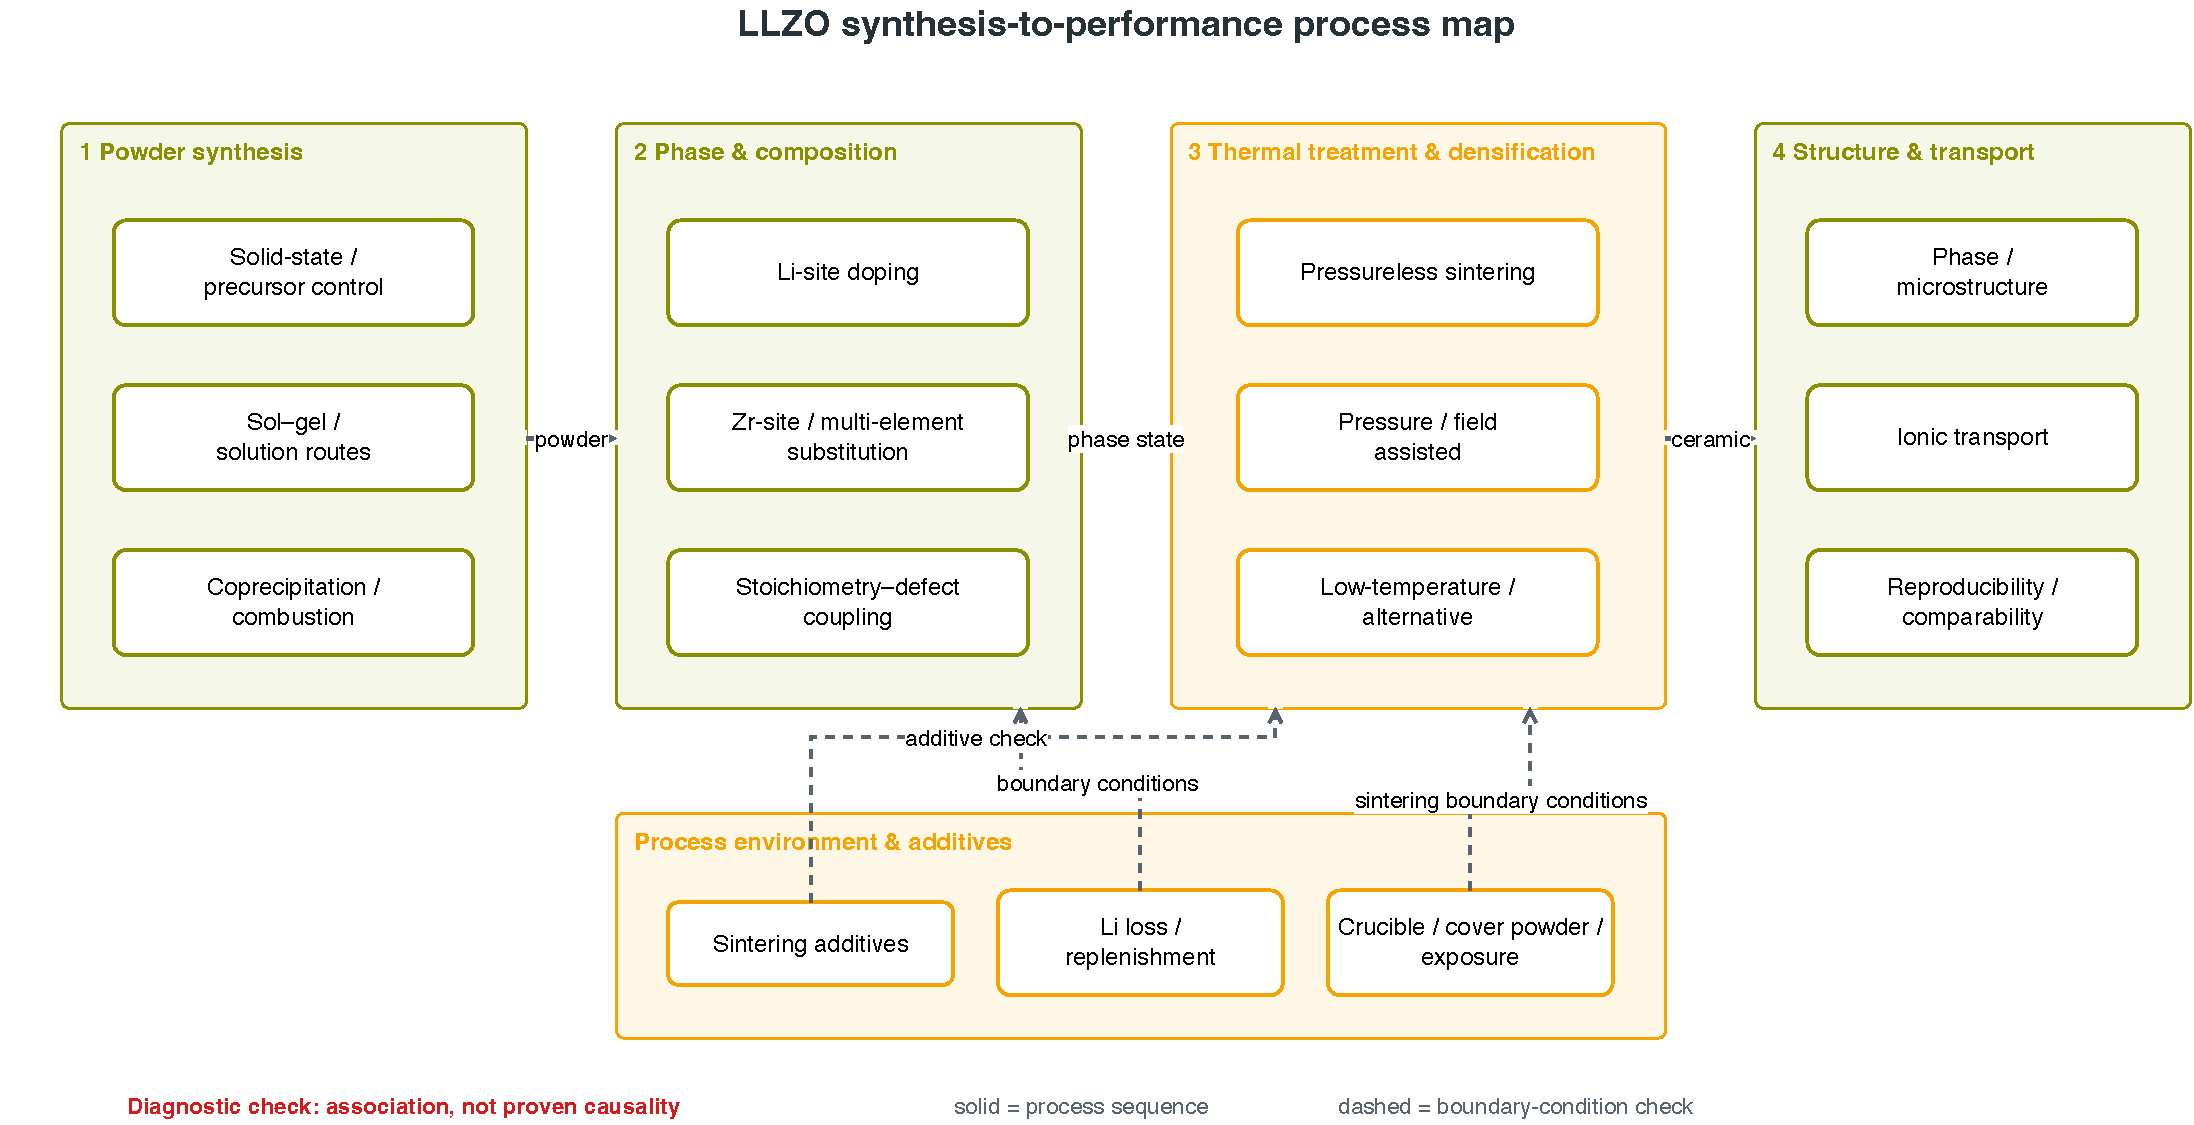
\includegraphics[width=\textwidth]{figures/pdf/llzo_process_map.pdf}
\caption{Faceted LLZO process map. Solid arrows encode group-level process order; dashed arrows encode boundary-condition checks involving lithium loss, crucible\slash exposure, and additives. The map identifies associations to inspect, not proven causal effects.}
\label{fig:process-map}
\end{figure*}

Three boundary tests make the framework operational. First, precursor control belongs to P1 when the controlled object is powder formation or mixing; composition and defect state belong to P2, while the same paper may retain both modifier and evidence tags. Second, ``low-temperature densification'' is a process objective in P3, whereas additive identity is an M4 modifier; a paper may legitimately carry both. Third, a modifier records what changed, while an evidence tag records what must be reported before the change can be compared.

Minimal phase and transport vocabulary is also necessary. The collection contains a computational abstract examining native defect populations as functions of synthesis conditions and explicitly challenging universal simple vacancy-compensation assumptions \cite{squires2019native}. Other audited records are title-level anchors for gallium-associated cubic-phase stabilization \cite{shinawi2013stabilization}, lithium stoichiometry in tetragonal LLZO \cite{ilina2014lithium}, and LLZO synthesis\slash thermodynamics \cite{aleksandrov2021superionic}. Because those three records are title-only locally, this review does not infer dopant occupancy, phase-transition values, or thermodynamic mechanisms from them. Likewise, total, bulk, and grain-boundary conductivity remain different observables; the word ``conductivity'' is not treated as a condition-complete comparison until type and test temperature are supplied.

The framework thus changes the reader's default question. Instead of asking which route wins, it asks which stage was deliberately varied, which modifiers moved with it, which readout was used, and which minimum-record fields remain available. That question recurs in every route discussion below.
